%%% PRomemoria, 20 pagine
APPUNTI:
-quando si allinea con il riferimento si vede 'solo' quello che c'è nel riferimento

\vspace{2cm}
Introduzione:
- allineamento usando la sequenza di riferimento, limiti nell'usare la sequenza di riferimento, approccio pangenomica.

Nella conversione di gfainvcf il core è l'identificazione delle bubble

Genoma di sars-cov2, focalizzarsi su TIME CONSUMING   


%Tabella  (scrivere meglio descrizioni )
%bubblePop & Bubble detection
%gfa2vcf &  rewrite file in gfa format in a vcf 
%gfa2allelefreq & explanation 
%gfa2genofreq & explanation 
%gfa2fst & explanation 
%devo spiegare nel dettaglio le funzioni in termine di codice o di cosa fanno? 
%Aggiungere anche mstovcf,seqgentogfa?

1. descrizione vgpop (6 pagine entro 5 giugno ) 
1a. Bubble detection
1b. variant calling 
1c. validation 
1d. allelic and genotipic frequencies, Fst 

2. application to simulated data (6 pagine entro 6 giugno) 
2a. simulation scenario and tools 
2b. application of vgpop to simulated data 

3. Study cases: (6 pagine) 


- covid19
allele frequencies from pangenome 
De-novo assembly
- yeast 
allele frequencies

% Chapter results

\chapter{Results achieved by the Candidate} % Main chapter title

\label{Chapter5} % For referencing the chapter elsewhere, use \ref{Chapter4} 

%----------------------------------------------------------------------------------------



%~~~~~~~~~~~~~~~~~~~~~~~~~~~~~~~~~~~~~~~~~~~~~~~~~~~~~~~~~~~~~~~~~~~~~~~~~~~~~~~~~~~~~~~


%%%%%%%%%%%%%%%%%%%%%%%%%%%%%%%%%%%%%%%%%%%%%%%%%%%%%%%%%%%%%%%%%%%%%%%%%%%%%%%%%%%%%%%
%  Section 
%%%%%%%%%%%%%%%%%%%%%%%%%%%%%%%%%%%%%%%%%%%%%%%%%%%%%%%%%%%%%%%%%%%%%%%%%%%%%%%%%%%%%%%

%\section{Description vgpop}
\section{Implementation of the \vgp library}  

I developed a library named \vgp to conduct standard population genetics analyses using pangenomic data models. Typically represented in the Graphical Fragment Assembly (GFA) format, these models can represent whole genome alignments in a compact graphical structure. The library is written in Python programming language under MIT license; the code is publicly available on GitHub (\url{https://github.com/Flavia95/VGpop}) 

At its present state \vgp contains five functions briefly introduced in tab \ref{tab:functionvgpop} and detailed in the following paragraphs.

\vspace{1cm}

{\small
\begin{table}[H]
\caption{Functions implemented in \vgp}
\label{tab:functionvgpop}
\centering
\begin{adjustbox}{width=0.80\textwidth}
\begin{tabular}{c c c c }
\toprule
\tabhead{vgpopfunction} & \tabhead{Description} & Input & Output \\
\midrule
bubblepop & Identification of polymorphic genomic regions (bubbles) &  GFA & dictionary  \\
gfa2vcf & Conversion of files in GFA format to VCF format & GFA & VCF \\
gfa2allelefreq & Calculation of allele frequencies & GFA & allelefreqfile \\
gfa2genofreq & Calculation of genotype frequencies & GFA & genotypefrequenciesfile \\
gfa2fst & Calculation of F\textsubscript{ST} & GFA & fstfile\\
\bottomrule\\
\end{tabular}
\end{adjustbox}
\end{table}
}

%\vspace{1cm}

%%%%%%%%%%%%%%%%%%%%%%%%%%%%%%%%%%%%%%%%%%%%%%%%%%%%%%%%%%%%%%%%%%%%%%%%%%%%%%%%%%%%%%%%%%%%
%  Subsection 
%%%%%%%%%%%%%%%%%%%%%%%%%%%%%%%%%%%%%%%%%%%%%%%%%%%%%%%%%%%%%%%%%%%%%%%%%%%%%%%%%%%%%%%%%%%%


\subsection{Bubblepop}

The main challenge of my project was to extract the information about variable sites (i.e. regions where more that one type of sequence is present) from the graphs. Any population genetic analysis is in fact based on the information contained in the variable segments of the sequence and their occurrence in the population under investigation. Because of their appearance in the pangenome graph, variable sites are referred to as bubbles (Figure \ref{fig:gfa.png}). \\

The core of \vgp is the \bbp function, which takes as input a pangenome, detects bubbles, and outputs the sequences of the variants contained in the bubbles.

\bbp takes as input a GFA file and gives as output a dictionary, i.e. a table of correspondences between region of the graph and sequence variants. It explores the graph using the two recursive algorithms described in the following paragraphs and works in two consecutive steps. 

%% non servono le lettere, zzom dalontano, graph piu' complesso senza dettaglio si fa vdere DFS sceglie un nodo  eesplora a casa un pezzoee  
%tree con root piu' lontana, aggiungere un pezzo di root 

\begin{figure}[H]
\centering
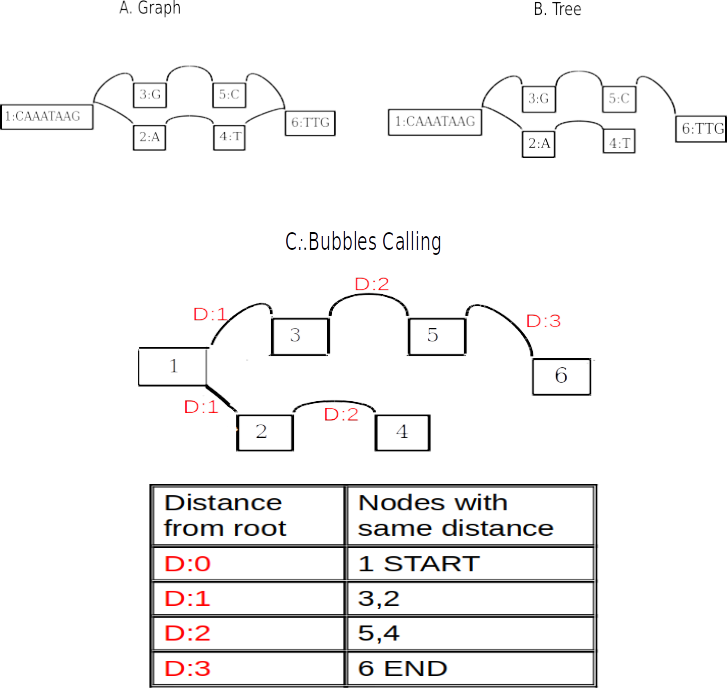
\includegraphics[width=1.00\textwidth]{fig/bubblepop.png}
\decoRule
\caption{\textit{bubblepop} transforms a pangenome (\textbf{A}) in a tree (\textbf{B}) using two algorithms, the Depth First Search and the Breadth first Search. On tree identify bubble (\textbf{C})}
\label{fig:bubblepop.png}
\end{figure}


\setcounter{secnumdepth}{3}
\subsubsection{Step 1: Depth first Search}

%I use two recursive algorith \cite{geeksforgeeks.org}.%questo e' un sito generico
The Depth First Search (DFS) \cite{korf1985depth,wiki:DFS} is a recursive algorithm for searching graph data structures. DFS select an arbitrary node as root node and explores as far as possible along each branch. The exploration process runs until some depth cutoff is reached, and then DFS backtracks to the next most recently expanded node. Therefore, only the path of nodes from the initial  node to the current  node  must be stored in order to execute the algorithm (Figure \ref{fig:bubblepop.png}A))

%vertex==node? non capisco questo paragrafo
DFS marks each vertex of a graph as visited. With this, start by one of the vertices of the graph in a stack. Take the item on top of the stack and add it to the list visited. Create a list of the adjacent nodes of that vertex. Add node that is not in the visited list.\\

In \bbp I use the DFS algorithm to explore the graph starting from a random node of the pangenome. At each iteration, \bbp creates a spanning tree from the part of the pangenome that is explored (Figure \ref{fig:bubblepop.png}B), threfore transforming the pangenome in a set of trees.\\ %vediamo meglio questo: Starting from the pangenome graph, with the DFS algorithm a spanning tree of its vertices is obtained.\\

A tree is an entity that describes relationships between objects (Figure \ref{fig:phylogenies.jpg}). The tips of the tree are called leaves; leaves are connected by branches, whose length is proportional to the observed differences between the leaves; the coalescence of two branches generates a node or vertex. In phylogeny and evolutionary genetics the nodes indicate the most common ancestor of sequences. In trees obtained from pangenomes, the branches are obtained by resolving the bubble in its edges components and the nodes represent chunks of sequences, the root of the tree is a special node located at the beginning of the tree. 

%aggiungere due colori uno per pangenomica uno per evolutonary, la figura serve per ora e per dopo
\begin{figure}[H]
\centering
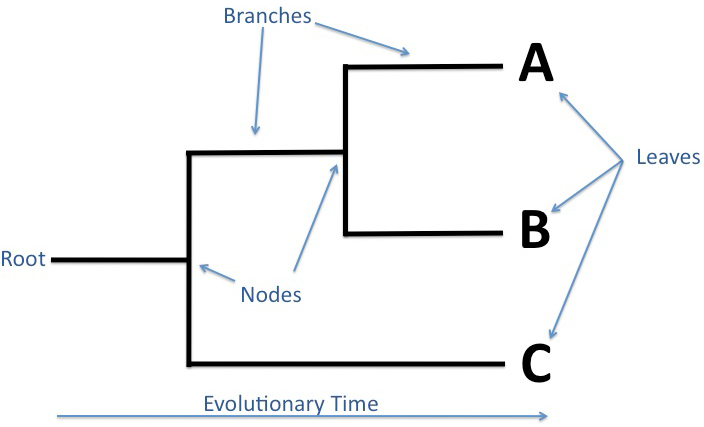
\includegraphics[width=0.80\textwidth]{fig/phylogenies.jpg}
\decoRule
\caption{\textbf{Fig: phylogenetic tree}. 
\url{modified from https://arthropoda.wordpress.com/2010/01/19/introduction-to-phylogenetics/}}
\label{fig:phylogenies.jpg}
\end{figure}

\subsubsection{Step 2: Breadth first Search}
Breadth First Search (BFS) \cite{beamer2012direction} is another recursive algorithm for traversing or searching tree or graph data structures. I used BFS on the trees obtained applying DFS (Figure \ref{fig:bubblepop.png}B).

When used on trees, at each iteration BFS starts at the tree root and explores all of the neighbor nodes at one step, then expands to the nodes at the next steps until a goal state is reached \cite{korf1985depth, wiki:BFS}. The information encountered during the exploration is recored. 
%come per BFS quest aparte no nmi e' chiara, no capisco cosa vuoi dire, da migliorare 
With this start by putting any one of the three's vertices at the back of a queue.Take the front item of the queue and add it to the visited list. Create a list of that vertex's adjacent nodes. Add the ones which aren't in the visited list to the back of the queue. \url{https://www.programiz.com/dsa/graph-dfs}

In \bbp, I used BFS to the trees obtained by DFS (Figure \ref{fig:bubblepop.png}B).
%distance of a.... leave?
In particular with BFS I calculated the distance of a node from the root node of the tree and stored this information in a dictionary, i.e. a table of correspondence (Figure \ref{fig:bubblepop.png}). 

%%%%% IMPORTANTE: tutt ala perte di come ordini le bubbles e scegli il riferimento?? in pratica la ricostruzione della sequenza? 






%%%%%%%%%%%%%%%%%%%%%%%%%%%%%%%%%%%%%%%%%%%%%%%%%%%%%%%%%%%%%%%%%%%%%%%%%%%%%%%%%%%%%%%%%%%%
%  Subsection 
%%%%%%%%%%%%%%%%%%%%%%%%%%%%%%%%%%%%%%%%%%%%%%%%%%%%%%%%%%%%%%%%%%%%%%%%%%%%%%%%%%%%%%%%%%%%


\subsection{gfa2vcf}
%tolto the second, non c'e un ordine 
The \textit{gfa2vcf} function of \vgp takes as input a graph in the GFA format and output a corresponding linear representation in the VCF format. To do this \textit{gfa2vcf} uses first \bbp, and then \bbc a function that make explicit the content of the bubbles and its position along a chosen reference sequence.    
I used the information contained in the dictionary produced using \bbp to transform the information of the graph in a linear format. 


\setcounter{secnumdepth}{3}
%forse questo paragrafo serve qui? 
\subsubsection{\bbc}
Once the pangenome has been decomposed with \bbp in a set of trees whose information are stored in dictionary, \bbp make explicit the content of the bubbles and its position along a chosen reference sequence.    

Within the dictionary, the beginning and the end nodes of a bubbles are identified by the fact that their distance from the root is uniqe, i.e. they are the only nodes with a specific distance from the tree. (Figure \ref{fig:bubblepop.png}C). All other nodes are  inner nodes of bubbles and correspond to variable regions of the sequence, furthermore nodes with the same distance from the root are in the same bubble. 





\subsubsection{Extracting Variant}
%"""QUESTO È VARIANT CALLING, QUINDI NON VA BENE"""Variant calling is the process of identifying genetic variants. First, sequence reads from one individual are aligned against the reference genome, then variable sites are identified as the ones where the sequence differs from the reference genome.

\begin{itemize}
\item\textbf{Possible paths}

Considering all the possible paths, the variants have been called respect to a path chosen as reference. A variant is a nodes supported by at least one path, whose sequence is different from the sequence of the corresponding node in the chosen reference.

\item\textbf{SNV and INDEL}

For Deletion if the considerate node in the REF is the current node in the current path, it means that in the current path a node is missing, so there is a deletion respect to the REF.
For Insertion if the considerate node in the current path is the current node in the ref, it means that in the current path there is a node that is missing in the REF, that is an insertion.

For SNV if the sequence are different in the current path respect to the REF.
\end{itemize}

I obtained VCF.


%va completata con una parte che fa vedere il GFA e se vuoi il VCF risulatante da questa bolla
\begin{figure}[H]
\centering
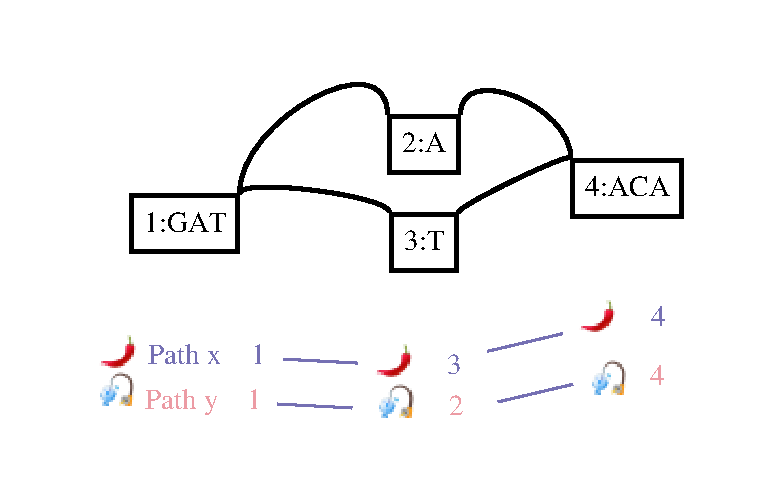
\includegraphics[width=1.10\textwidth]{fig/GraphchrXnew.pdf}
\decoRule
\caption{\textbf{Fig A: Bubble}. Path x represents the sequence used as a reference to describe variants that are present in a sequence analysed.} %aggiungere path
\label{fig:bubble.png}
\end{figure}

\begin{figure}[H]
\centering
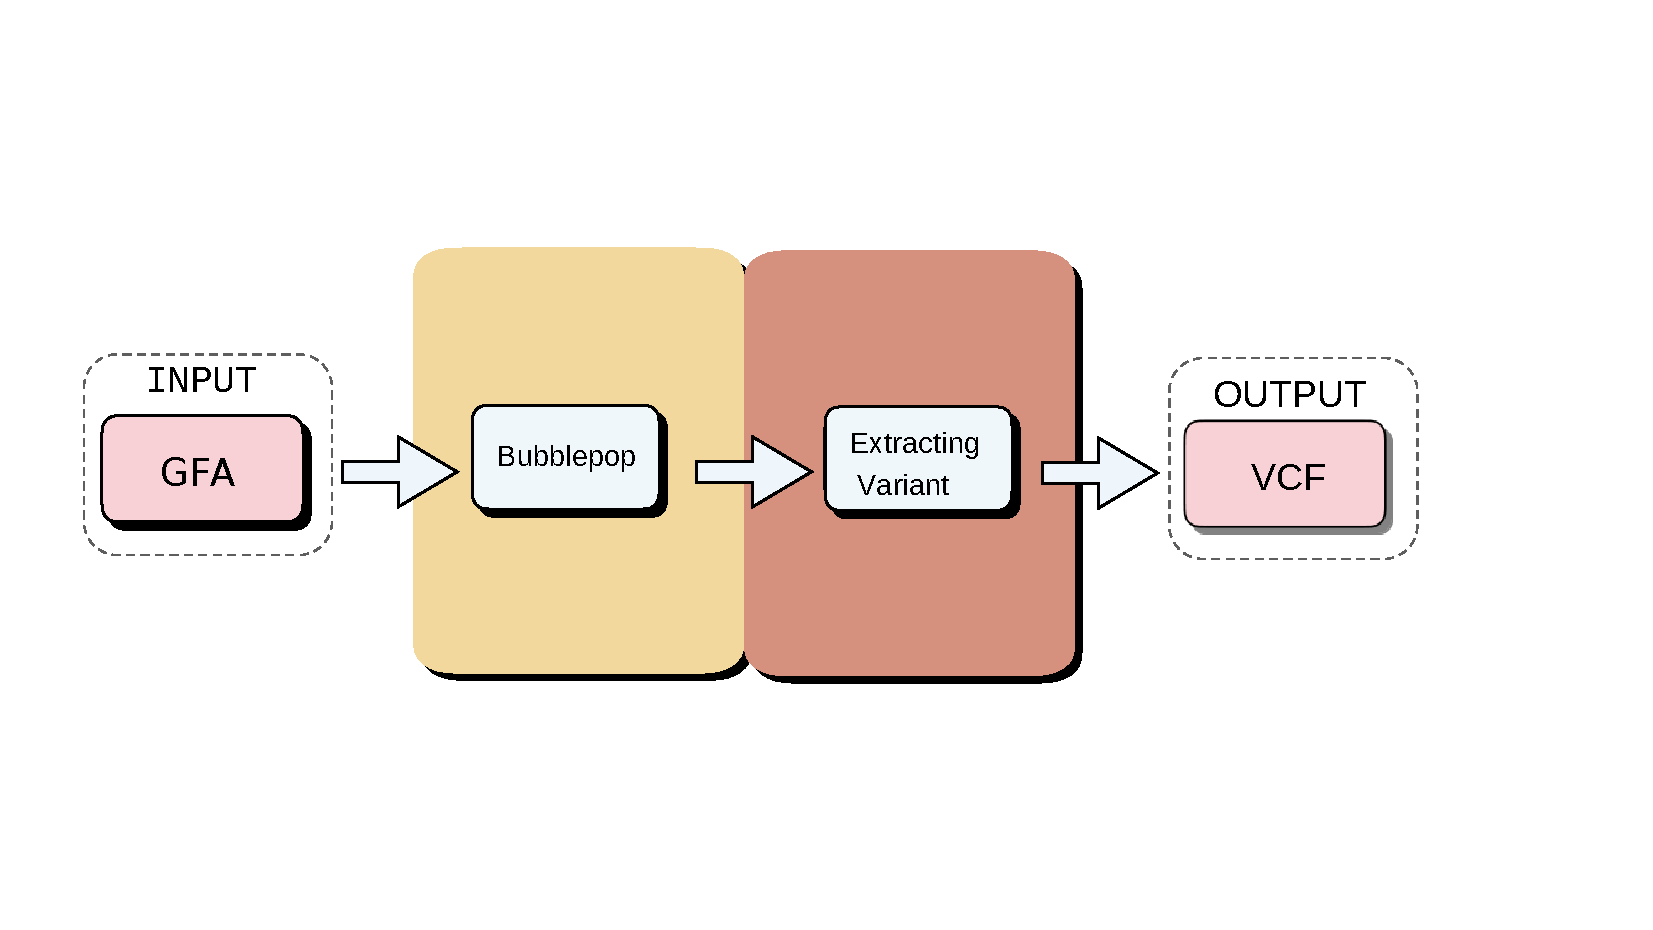
\includegraphics[width=1.10\textwidth]{fig/gfatovcfnew.pdf}
\decoRule
\caption{\textbf{Graph} GfatoVcf}
\label{fig:vgpop.pdf}
\end{figure}



{\small
\begin{table}
\caption{gfa2vcf}
\label{tab:gfatovcf}
\centering
\begin{adjustbox}{width=0.50\textwidth}
\begin{tabular}{c c}
\toprule
\tabhead{GFA} & \tabhead{VCF} \\
\midrule
 Path Name & CHROM \\
 Length of sequence & POS \\
 Path Chose & REF \\
 Center of bubble & ALT \\
 SNV, INDEL & Type\\
\bottomrule\\
\end{tabular}
\end{adjustbox}
\end{table}
}

%%%%%%%%%%%%%%%%%%%%%%%%%%%%%%%%%%%%%%%%%%%%%%%%%%%%%%%%%%%%%%%%%%%%%%%%%%%%%%%%%%%%%%%%%%%%
%  Subsubsection 
%%%%%%%%%%%%%%%%%%%%%%%%%%%%%%%%%%%%%%%%%%%%%%%%%%%%%%%%%%%%%%%%%%%%%%%%%%%%%%%%%%%%%%%%%%%%

\subsubsection{Validation of the VCF obtained with \textit{gfa2vcf}}

For validation VCF I use (\url{https://nicedoc.io/vgteam/vg}) Variation graphs provide a succinct encoding of the sequences of many genomes. 
A variation graph (in particular as implemented in vg) is composed of:
\begin{itemize}
\item nodes: which are labeled by sequences and ids
    
\item edges: which connect two nodes via either of their respective ends
   
\item paths: describe genomes, sequence alignments, and annotations (such as gene models and transcripts) as walks through nodes connected by edges

Tools in vg maintain paths as immutable during transformations of the graph. They use paths to project graph-relative data into reference-relative coordinate spaces. Paths provide stable coordinates for graphs built in different ways from the same input sequences.

\end{itemize}
I used vg tool (adapted from \cite{vg}) to work with genome variation graphs for validate the VCF files obtained with the \textit{gfa2vcf} function. To date, the first path in the GFA file is used as reference; in the next updates, it will be possible to set any available paths.
GFAstart(\ref{fig:validationgraph.png}A), is the input of \textit{gfa2vcf} function, and output of this function i.e VCF format is the input of the following commands.  

As output of vg I obtained GFA (\ref{fig:validationgraph.png}B, ) similar to GFAstart. 

\textit{gfa2vcf} works well. 



\begin{figure}[H]
\centering
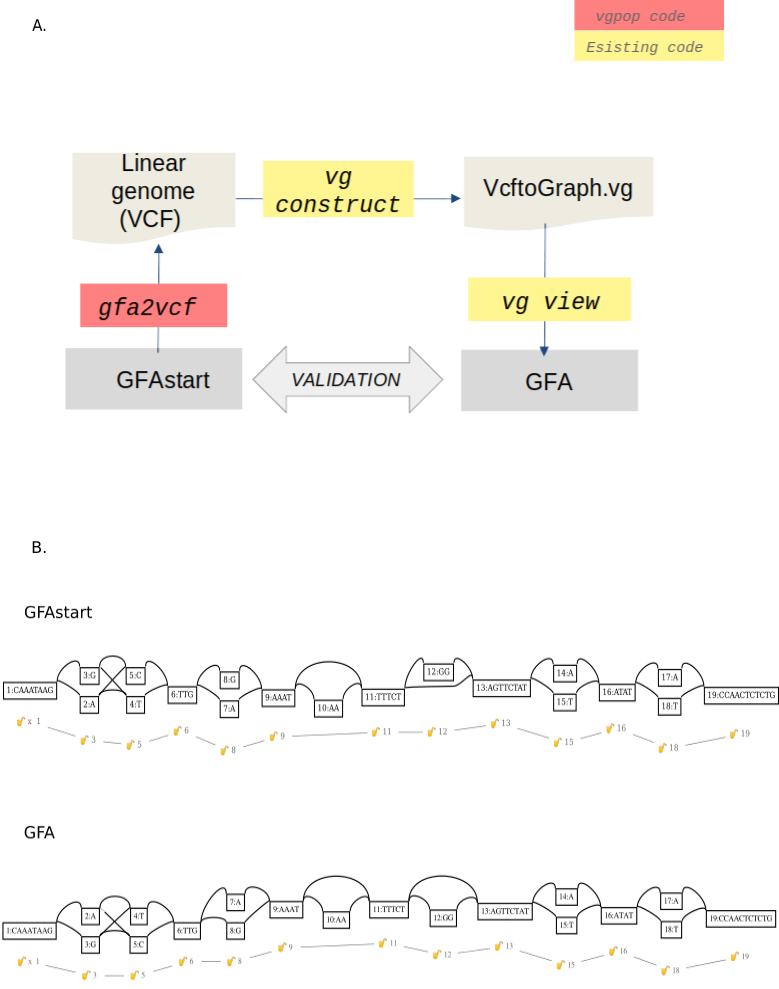
\includegraphics[width=1.00 \textwidth]{fig/validationgfa2.vcf.png}
\decoRule
\caption{\textit{gfa2vcf} transforms a GFAstart in VCF.I use this for validate this result(\textbf{A}). GFAstart end GFA are equal (\textbf{B})}
\label{fig:validationgraph.png}
\end{figure}

%%%%%%%%%%%%%%%%%%%%%%%%%%%%%%%%%%%%%%%%%%%%%%%%%%%%%%%%%%%%%%%%%%%%%%%%%%%%%%%%%%%%%%%%%%%%
%  Subsection 
%%%%%%%%%%%%%%%%%%%%%%%%%%%%%%%%%%%%%%%%%%%%%%%%%%%%%%%%%%%%%%%%%%%%%%%%%%%%%%%%%%%%%%%%%%%%

\subsection{gfa2allelefreq} 

Allele frequency gives us indication on how common an allele is in a population. It is calculated by counting how many times the allele appears in the population, dividing by the total number of copies of the gene.

Haploids    $p = \dfrac{i}{N}$

Diploids   

frequency of A $p = {f(AA)} + \dfrac{1}{2} f(AB)$

frequency of B $q = {f(BB)} + \dfrac{1}{2} f(AB)$

The third function of \vgp is the \textit{gfa2allelefreq} , which takes as input a GFA format, and as output a file that contains the calculation of allele frequencies.
In this specific case I obtained two file of calculation, one from each population. 

This calculation start with \textit{bubblepop}, after detection of bubble I calculate allele frequencies, for each variants the number of  paths  are  calculate  that  support  the  variant node divided  by  total  number  of  paths(considered even REF).
Only allele frequencies different from 1 were considered. 
 

%%%%%%%%%%%%%%%%%%%%%%%%%%%%%%%%%%%%%%%%%%%%%%%%%%%%%%%%%%%%%%%%%%%%%%%%%%%%%%%%%%%%%%%%%%%%
%  Subsection 
%%%%%%%%%%%%%%%%%%%%%%%%%%%%%%%%%%%%%%%%%%%%%%%%%%%%%%%%%%%%%%%%%%%%%%%%%%%%%%%%%%%%%%%%%%%%


\subsection{gfa2genfreq}

The fourth function of \vgp is the \textit{gfa2genfreq}, which takes as input a GFA format, and as output a file that contains the calculation of genotype frequencies.

Genotype frequencies \cite{brooker2014principles} in a population is the number of individuals with a given genotype divided by the total number of individuals in the population. In population genetics, the genotype frequency is the frequency or proportion of genotypes in a population. 

$f(a) = \dfrac{(Aa) + 2 x (aa))}{2 x (AA) + 2 x (Aa) + 2 x (aa)}$

I counted ATGC in a position and I checked the reference base and calculate for each allele the frequency (count/numhaplotype).


%%%%%%%%%%%%%%%%%%%%%%%%%%%%%%%%%%%%%%%%%%%%%%%%%%%%%%%%%%%%%%%%%%%%%%%%%%%%%%%%%%%%%%%%%%%%
%  Subsection 
%%%%%%%%%%%%%%%%%%%%%%%%%%%%%%%%%%%%%%%%%%%%%%%%%%%%%%%%%%%%%%%%%%%%%%%%%%%%%%%%%%%%%%%%%%%%


\subsection{gfa2fst}

The fifth function of \vgp is the \textit{gfa2$F\textsubscript{st}$}, which takes as input allele frequencies file, and as output a file that contains the calculation of $F\textsubscript{st}$.

The fixation index is a measure of population differentiation due to genetic structure. It is frequently estimated from genetic polymorphism data, such as single-nucleotide polymorphisms (SNP) or microsatellites developed as a special case of
the Wright’s fixation index ($F\textsubscript{st})$ is a measure of population differentiation due to genetic structure. 

It can be estimated as the standardized variance of allele frequencies among sub-populations.

$F\textsubscript{st} = \dfrac{s^{2}}{p(1-p)}$

with s and p being the variance and mean, respectively, of the allele frequency. 

$F\textsubscript{st}$ \cite{barbujani2010human} ranges from 0, when all sub-populations are identical, to 1, when different alleles are fixed in different sub-populations.


The central points of this function are three:



\begin{itemize}
\item\textbf{Mean of  allele frequencies}:  obtained by \textit{gfa2allelefreq} from two populations. These frequencies represent 
\begin{verbatim}
mean = statistics.mean([freq_pop1, freq_pop2])
\end{verbatim}
 
\item\textbf{Calculation of $F\textsubscript{st}$}

\begin{verbatim}
fst = statistics.pvariance([freq_pop1, freq_pop2])/((mean)*(1-mean))
\end{verbatim}
\item\textbf {Mean of $F\textsubscript{st}$} from 100 replicate. 

\begin{verbatim}
mean_fst_list.append(statistics.mean(fst_list))
\end{verbatim}
\end{itemize}




\vspace{8cm}


%%%%%%%%%%%%%%%%%%%%%%%%%%%%%%%%%%%%%%%%%%%%%%%%%%%%%%%%%%%%%%%%%%%%%%%%%%%%%%%%%%%%%%%
%  Section 
%%%%%%%%%%%%%%%%%%%%%%%%%%%%%%%%%%%%%%%%%%%%%%%%%%%%%%%%%%%%%%%%%%%%%%%%%%%%%%%%%%%%%%%

\section{Application to simulated data}
I exploited analyses of genetic population on simulated data to already know what to expect.


%%%%%%%%%%%%%%%%%%%%%%%%%%%%%%%%%%%%%%%%%%%%%%%%%%%%%%%%%%%%%%%%%%%%%%%%%%%%%%%%%%%%%%%%%%%%
%  Subsection 
%%%%%%%%%%%%%%%%%%%%%%%%%%%%%%%%%%%%%%%%%%%%%%%%%%%%%%%%%%%%%%%%%%%%%%%%%%%%%%%%%%%%%%%%%%%%

\subsection{Simulation Scenario and Tools}

\subsubsection{MS}

I used MS \cite{hudson2004ms}, a program to generate samples under a variety of neutral models. The purpose of this program is to allow one to investigate the statistical properties of such samples, to evaluate estimators or statistical tests, and generally to aid in the interpretation of polymorphism data sets.

The program ms can be used to generate many independent replicate samples under a variety of assumptions about migration, recombination rate and population size. I simulated two populations that are divided into three different times. I expected Fst to be greater for the two populations more distantly divided over time.(T3)

%forse citare nei metodi pacchetto usato per fare i plot?




\begin{figure}[H]
\centering
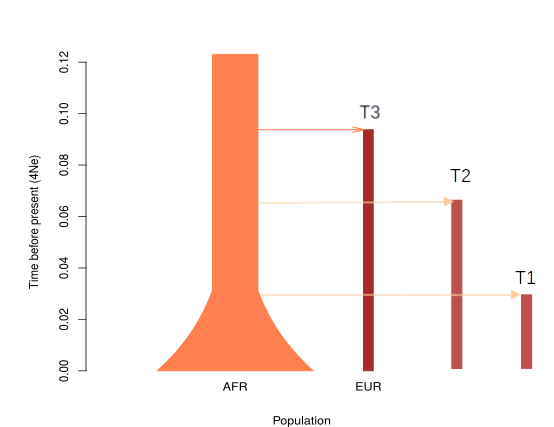
\includegraphics[width=1.10\textwidth]{fig/populationthreetime.png}
\decoRule
\caption{\textbf{Fig:Population}. 
T1 (0.031254 Ne), T2(0.0625 Ne),T3(0.09375 Ne)}
\label{fig:population.pdf}
\end{figure}

\begin{verbatim}
In the first case I simulated two populations that divided 5.000 generations ago.


ms 80 100 -t 11.2 -I 2 40 40 -g 1 44.36 -n 2 0.05 -eg 0.03125 1 0.0 -ej 0.03125 2 1   

I simulated two populations that divided 10.000 generations ago.

ms 80 100 -t 11.2 -I 2 40 40 -g 1 44.36 -n 2 0.05 -eg 0.03125 1 0.0 -ej 0.0625 2 1   

I simulated two populations that divided 15.000 generations ago.

ms 80 100 -t 11.2 -I 2 40 40 -g 1 44.36 -n 2 0.05 -eg 0.03125 1 0.0 -ej 0.09375 2 1   
\end{verbatim}

Explanation the parameters of ms:

\begin{itemize}
\item\textbf{nsam<nsample>:}
is the number of copies of the locus in each sample.

\item\textbf{nrep<nreplicate>:}
is the number of independent samples to generate;


\item\textbf{t <mutationrate>:}
is equal to $$4N0\mu$$ where N0 is the diploid population size and where u is the neutral mutation rate for the entire locus;

\item\textbf{I <individual>:}
followed by the number of subpopulations,npop, and the sample configuration. The sample configuration is a list of npop integers (n 1 n 2...) indicating the number of chromosomes sampled from each subpopulation;

\item\textbf{g <growth>:}
 it indicate the growth of pop1 at a definite time;

\item\textbf{n:}
it set growth of population 2 at time; 

\item\textbf{eg <growth rate>:}
pop1 stop growing at time 0.03125;

\item\textbf{ej <join>:}
Pop1 join with pop2. It is the parameter that change in three command. 

I convert mstogfa but I need the information about the links between the bubbles.  

\subsubsection{Seq-Gen}
I needed the whole sequence rebuilt and the links between the bubbles """SPIEGARE PERCHE' E/O PER FARCI COSA.

Seq-Gen \cite{rambaut1997seq} is a program that will simulate the evolution of nucleotide sequences along a phylogeny, using common models of the substitution process. A range of models of molecular evolution are implemented, including the general reversible model. 

Seq-Gen requires a tree as input, therefore I added the parameter -T to all the MS commands to obtained a tree as output. With seq-gen, I reconstructed the sequences for the three different simulated times.

\begin{verbatim}
seq-gen -mHKY -l 40 -s .2 -wa -z 783763255346462154 <treems40popT1> T1.seqgen

seq-gen -mHKY -l 40 -s .2 -wa -z 783763255346462154 <treems40popT2> T2.seqgen

seq-gen -mHKY -l 40 -s .2 -wa -z 783763255346462154 <treems40popT3> T3.seqgen

\end{verbatim}

Explanation of parameters:

\begin{itemize}

\item\textbf{m <MODEL>:} This option sets the model of nucleotide or amino acid substitution.
\item\textbf{l <SEQUENCELENGTH>:} This option allows the user to set the length in nucleotides or amino acids that each simulated sequence should be.
\item\textbf{s <SCALE>:} This option allows the user to set a value with which to scale the branch lengths in order to make them equal the expected number of substitutions per site for each branch. Basically Seq-Gen multiplies each branch length by this value.
\item\textbf{z <RANDOMNUMBERSEED>:} This option allows the user to specify a seed for the random number generator. Using the same seed (with the same input) will result in identical simulated datasets. This is useful because you can then delete the (often large) simulated sequence files to save disk space. To recreate a set of simulations, you must use exactly the same model options. The default is to obtain a seed from the system clock which will be displayed on the screen allowing it noted down.
\item\textbf{wa:}
Write Ancestral Sequences. This option allows the user to obtain the sequences for each of the internal nodes in the tree obtained with ms 
\end{itemize}

\end{itemize}

\subsection{Application vgpop}
\begin{figure}[H]
\centering
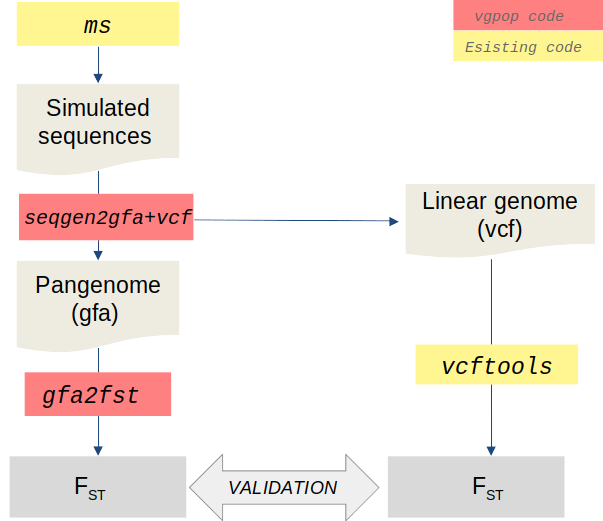
\includegraphics[width=1.00\textwidth]{fig/pipeline_new.png}
\decoRule
\caption{\textbf{Fig:Pipeline}. 
Validation.}
\label{fig:pipeline.pdf}
\end{figure}

Starting from ms, I obtained simulated sequences, I reconstruct an ancestral tree with Seq-Gen. 

These sequences were encoded in a GFA file and VCF file with \textit{seqgen2gfa+vcf }.


On GFA file I calculate the allele frequencies with \textit{gfa2allelefreq}, the genotype frequencies with \textit{gfa2genofreq}, and the Fst with \textit{gfa2fst}. 

On VCF file I extract individuals from the populations that I considered with bcftools. %non so se mettere questa parte
\begin{verbatim}

bcftools view -S pop_1.txt seqgen.vcf.gz -o seqgen.bcf.vcf.gz #pop1
bcftools view -S pop_2.txt seqgen.vcf.gz -o  seqgen.bcf.vcf  #pop2 
\end{verbatim}

Calculate Allele Frequencies for two populations with vcftools
\begin{verbatim}

vcftools --vcf seqgen.bcf.vcf --freq --out seqgen.bcf.pop1.vcf .frq

vcftools --vcf ms_rep{1}.bcf.vcf --freq --out seqgen.bcf.pop2.vcf.frq 

\end{verbatim}

I calculate Fst with \textit{vcf2fst} (aggiungerlo nell'immagine?). %aggiungere altre info sullo script

Fst is the same from GFA and VCF file.


\begin{figure}[H]
\centering
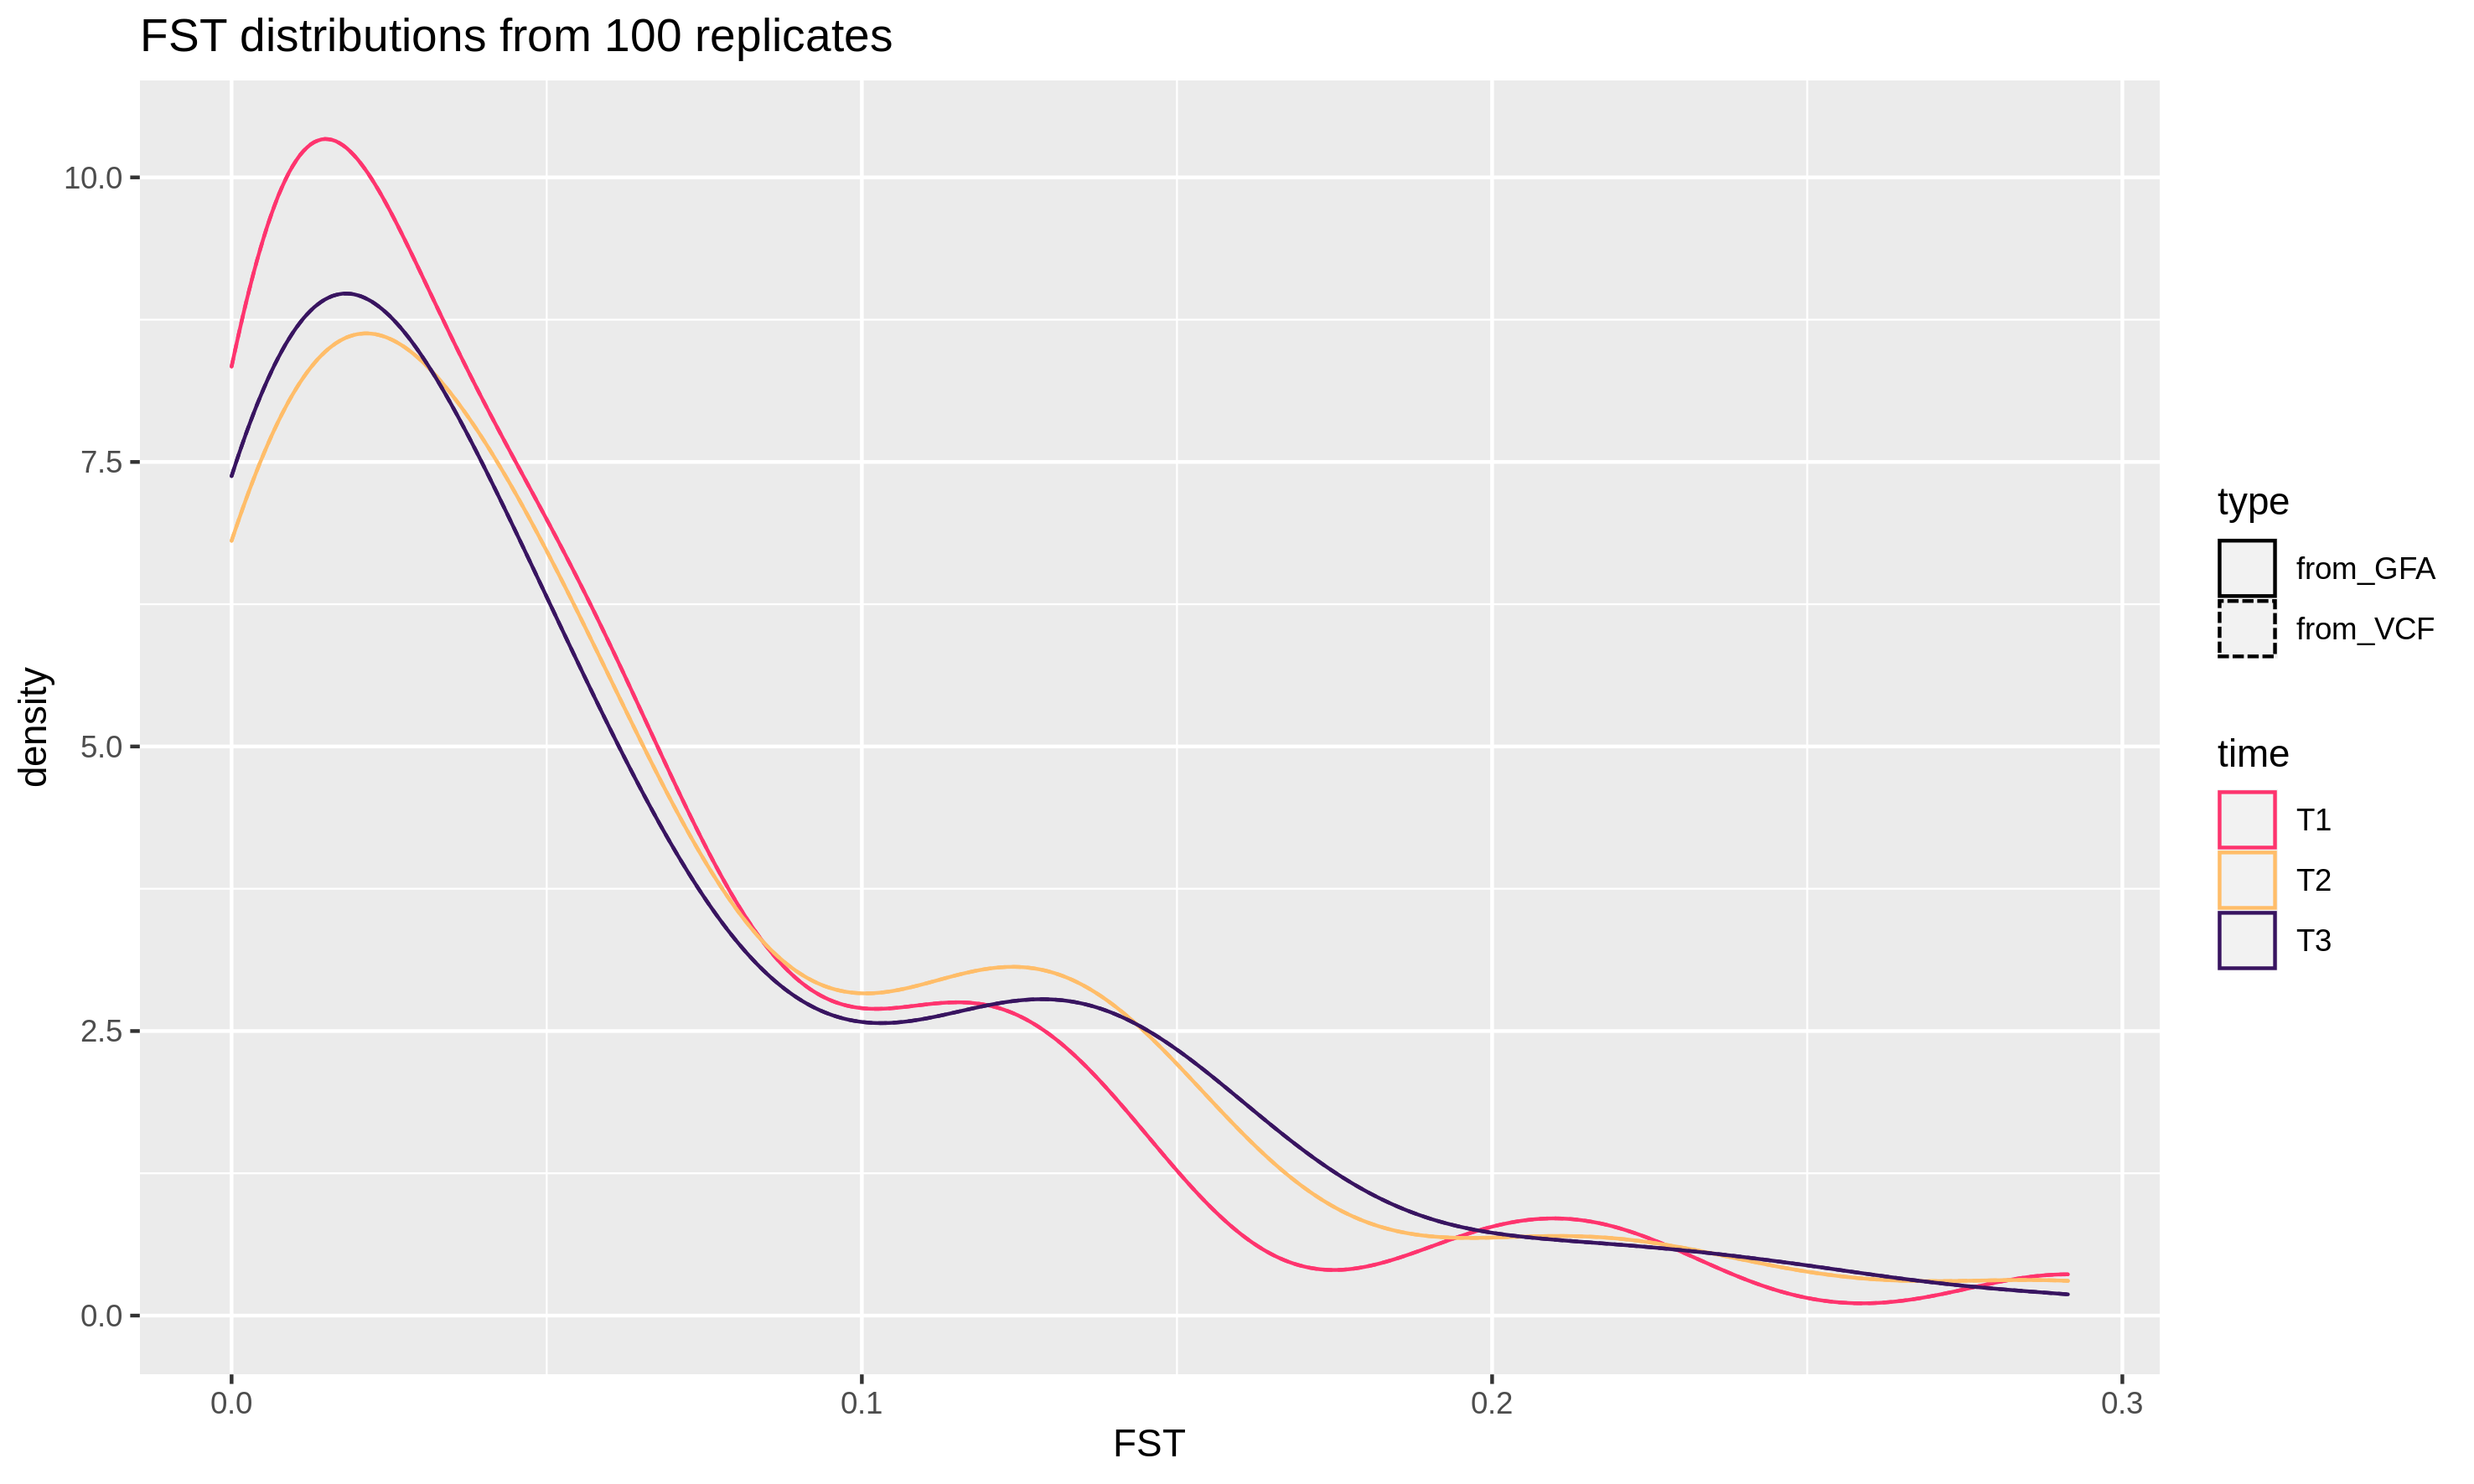
\includegraphics[width=1.00\textwidth]{fig/fst_time (1).png}
\decoRule
\caption{\textbf{Fig:valure of Fst are equal}.}
\label{fig:fsttime.png}
\end{figure}






\section{Study Cases}

I applicate two functions of \vgp to pangenomes of HLA. In particular I calculate \textit{gfa2vcf} and \textit{gfa2allelefreq}.

\subsection{Pangenome HLA}

\begin{figure}[H]
\centering
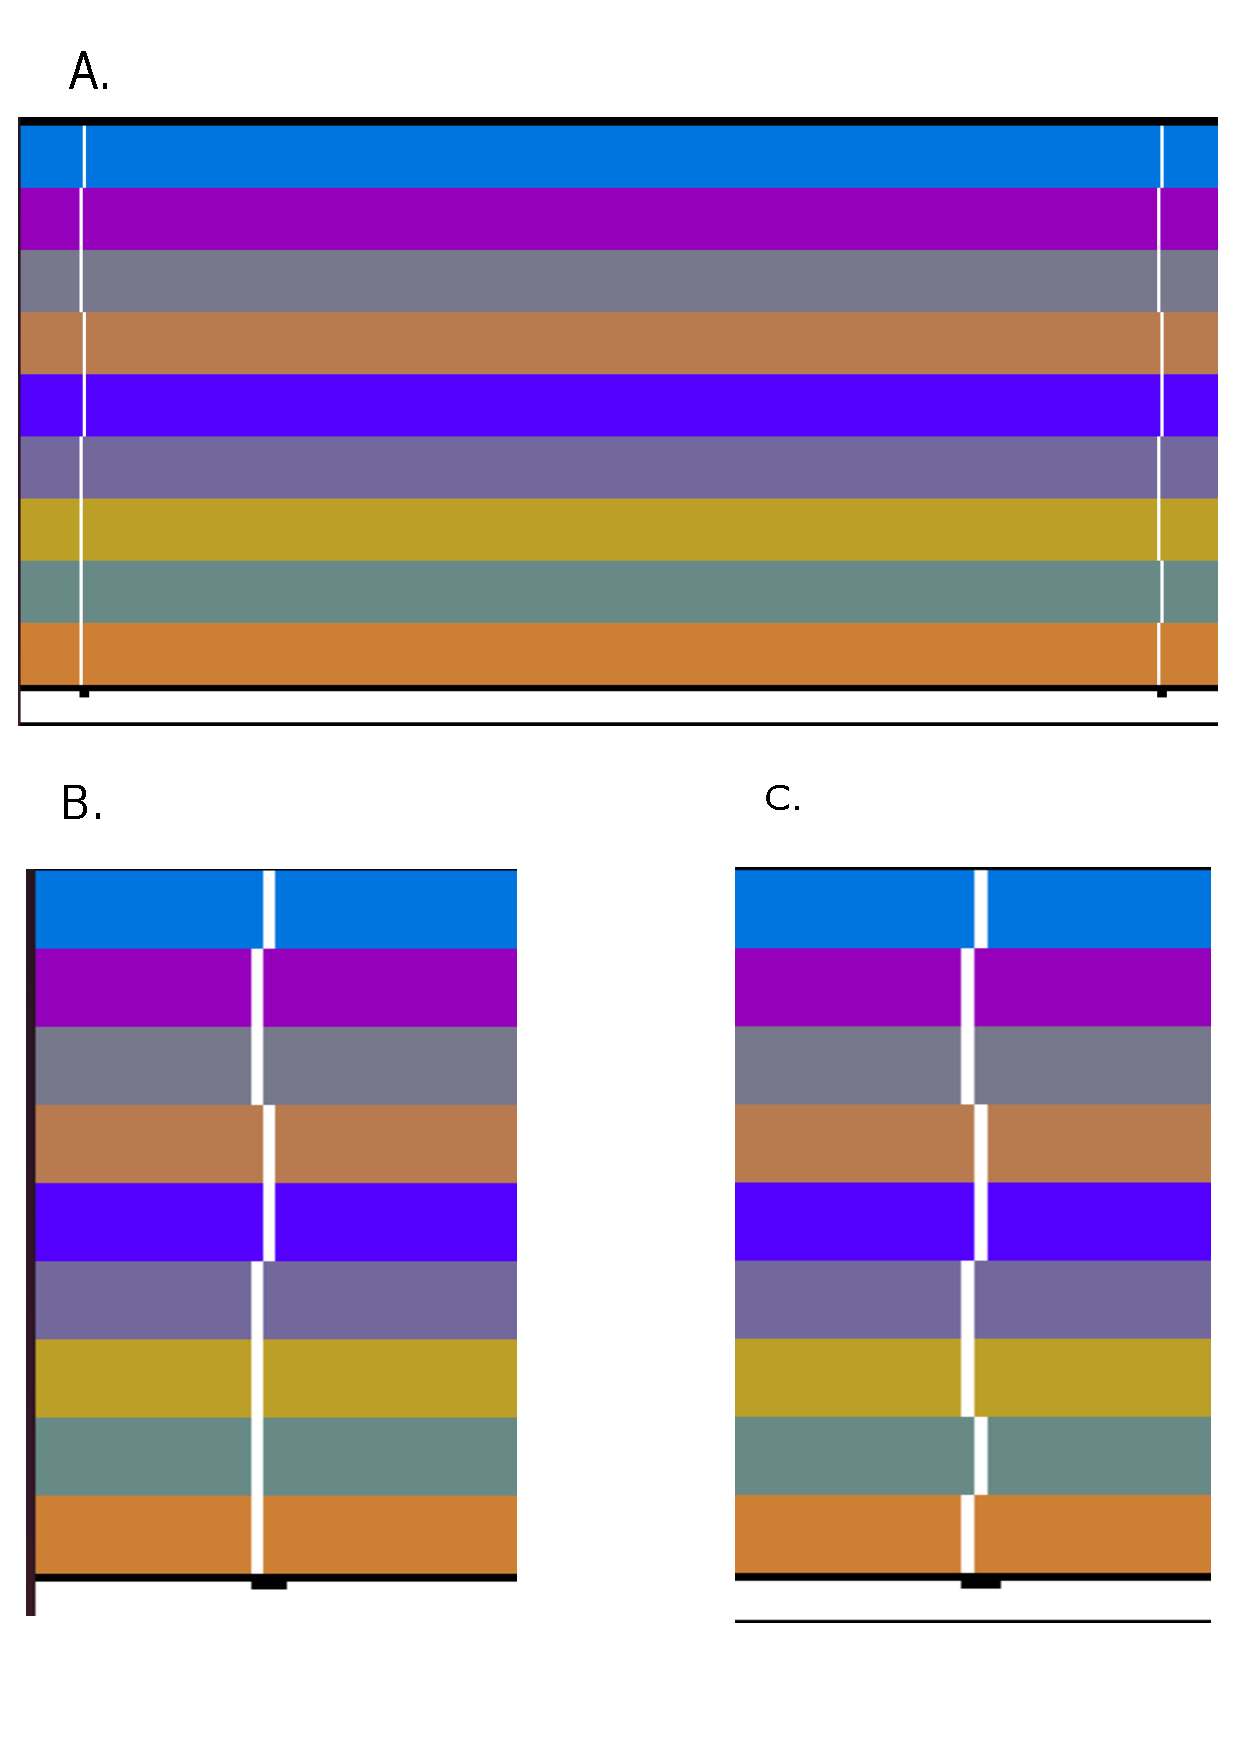
\includegraphics[width=0.50\textwidth]{fig/pangenome.pdf}
\decoRule
\caption{\textit{pangenome}. Is represented a piece of pangenome of HLA, the first row represent Reference and the other rows represent another paths. (\textbf{A}). Zoom for the first column  (\textbf{B}), zoom the second column(\textbf{C})}
\label{fig:pangenome.pdf}
\end{figure}


Pangenomic methods allow us to relate all genomes or sequences in our analysis directly to each other. One of the most polymorphic parts of the genome is the HLA region and for this thing I chose this region.

\subsection{gfa2vcf}

I build pangenome of HLA (see methods) and for the first time I calculate \textit{gfa2vcf}, I convert with odgi GFAformat in an odgiformat. I applicate this function and I obtained VCF.

\begin{verbatim}
odgi build -g E-3133.gfa -o E-3133.og
\end{verbatim}

For validate this result I use vg.
\begin{verbatim}
vg view -Fv E-3133.gfa > E-3133.vg
vg index E-3133.vg -x E-3133.xg
vg deconstruct -p "gi|568815592:30489405-30494204" E-3133.xg
\end{verbatim}

The results are the same.

\subsection{gfa2allelefreq}

The aim is calculate allele frequencies directly on a pangenome. \\

This calculation start with \textit{bubblepop}, after detection of  bubble I calculate allele frequencies, for each variants the number of paths are calculate that support the variant node divided by total number of paths (considered even REF).\\

In this figure ((\ref{fig:pangenome.pdf})A), the first row of the figure represent reference and other rows paths.
Fig: (\ref{fig:pangenome.pdf}A)  for the column in white: first row represent REF, the left node in the REF there isn't in six path, in fact for calculate allele frequencies six paths are divided with 9, the result is 0.66 (\ref{tab:gfa2freqandvcf}first row).


The same for the second column, left node there aren't in 5 paths, and for calculate allele frequencies I divided 5 paths for the total of paths i.e  9, the result is 0.56.


%sequenze nel pangenoma sotto forma di lettere


{\small
\begin{table}
\caption{gfa2freqandvcf}
\label{tab:gfa2freqandvcf}
\centering
\begin{adjustbox}{width=1.00\textwidth}
\begin{tabular}{c c c c c}
\toprule
\tabhead{CHROM} & \tabhead{POS} & \tabhead{REF} & \tabhead{ALT} & \tabhead{FREQ} \\
\midrule
gi|568815592:30489405-30494204 & 551 & 	T & C & 0.67\\
gi|568815592:30489405-30494204 & 883 & G & A & 0.56\\
gi|568815592:30489405-30494204 & 1141 & T & A & 0.11 \\
gi|568815592:30489405-30494204 & 3904 & G & A & 0.67\\
\bottomrule\\
\end{tabular}
\end{adjustbox}
\end{table}
}








